% -------------------------------------------------------------------------------------------------
% QUALITATIVE EVALUATION
% -------------------------------------------------------------------------------------------------
\section{Qualitative Evaluation}
\label{sec:qualitative_evaluation}
In this section, we will perform a qualitative evaluation of our solution with the other solutions,
such as full Virtual Machines and tools that implement the TOSCA standard. In our evaluation we
will compare the software required to provisioning the smart place infrastructure and also discuss
about the advantages of our solution compared with the others.

\subsection{Container-based vs. VM-based solution}
\label{sub:container_vs_vm_solution}
The provisioning of the RFID software in Cloud4Things is performed through Docker containers. The
decision to adopt this approach regards with the fact that we want our provisioned stack is as
small as possible, without the performance of our solution being affected. A alternative to
provisioning the RFID software stack is to use Virtual Machines. However, full VM presents
an overhead regarding the amount of resources that are consumed. In Figure \ref{fig:container_vs_vm}
we illustrate a comparison of the stacks between our solution and a full VM solution.

% Container vs. VM stack
\begin{figure}[!ht]
  \centering
  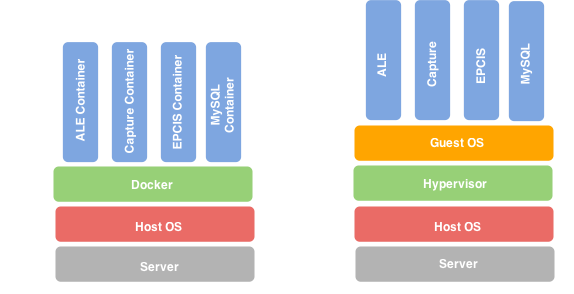
\includegraphics[width=.8\textwidth]{images/container-vs-vm-stack}
  \caption{Container vs. VM stack}
  \label{fig:container_vs_vm}
\end{figure}

The current implementation is running in a Amazon Linux based EC2 instance with a 8GB volume storage.
After provisioning the stack our implementation is using $\sim$2.6GB of the available storage, which $\sim$1.4GB
corresponding to the storage allocated by the Docker containers, as illustrated in Table \ref{table:containers_size}.

% Containers Size
\begin{table}[h]
\centering
\begin{tabular}{|c|c|}
\hline
\multicolumn{1}{|c|}{Container} & \multicolumn{1}{c|}{Size} \\ \hline
MySQL Database                  & 290 MB                    \\ \hline
EPCIS Repository                & 400 MB                    \\ \hline
Capture Application             & 381 MB                    \\ \hline
ALE Server                      & 390 MB                    \\ \hline
\end{tabular}
\caption{Docker containers size.}
\label{table:containers_size}
\end{table}

To compare our Docker-based approach with a full VM solution, we configure a Virtual Box VM running
Ubuntu 14.04 LTS with the software stack required to have a full installation of Fosstrak. Compared
with our implementation, a full VM approach requires almost twice the available storage - $\sim$4.7GB.

\subsection{Cloud4Things vs. TOSCA-based tools}
\label{sub:c4t_vs_tosca}

In order to provisioning the smart place infrastructure with TOSCA, we need to have a special
provisioning engine for TOSCA. Currently there are several tools that implements
a provisioning engine for TOSCA such as Ubuntu Juju\footnote{http://www.ubuntu.com/cloud/tools/juju},
Cloudify\footnote{http://getcloudify.org/} and the open-source implementation
OpenTOSCA\footnote{http://www.iaas.uni-stuttgart.de/OpenTOSCA/}.

These tools allow to modeling the application components in a more expressive way compared to using
only Chef. However TOSCA standard is not fully developed yet and does not support Container
technologies and the definition of monitoring services in the application topology.
